\section{Argument construction and result validation}\label{sec:C18:arguments}
Argument generation translates a task and its evidence into an executable object. The model must identify entities, select current values, satisfy cross-field constraints, and preserve exact strings where required. JSON syntax is the easiest part of this problem. A call can satisfy a schema while naming the wrong account, using a stale resource version, or combining fields that are individually valid but jointly inconsistent.

Use layered validation. The parser checks serialization. The schema checks types and required fields. The application checks domain preconditions and cross-field constraints. The authority monitor checks whether the operation is permitted. The remote service checks its current state. These layers should return distinguishable errors so the agent can repair the responsible field without broad speculative retries. A generic failure message can induce repeated changes to already correct arguments.

Constrained decoding can reduce malformed outputs by restricting token sequences to an allowed language. It does not establish that the selected entity or action is correct. It can also alter the behavior distribution used for training and likelihood accounting. If a rollout applies schema constraints, record them with the sampled output rather than recomputing probabilities under an unconstrained model. Syntactic reliability and statistical consistency interact at this interface.

Result validation likewise needs several levels. A parser can confirm that a returned object matches the declared type. A tool-specific validator can check a checksum, resource version, or test result. Semantic interpretation decides what the observation implies for the task. A language-model explanation generated by the tool is not automatically independent verification of the same model's action. Preserve raw evidence when it is needed to audit that inference.

One proposed argument-provenance record maps each consequential field to its source: direct user input, retrieved evidence, deterministic transformation, or model inference. This can be lightweight for read-only search queries and stricter for effects. If an identifier comes from an untrusted document rather than the authorized workspace, the dispatcher can detect the difference. The record does not make inferred values correct, but it makes their basis reviewable.

Evaluation should include near-valid errors. Test correct schemas with wrong identifiers, stale versions, units, boundary values, and conflicting fields. Include tools whose names are similar but whose effects differ. A benchmark containing only malformed JSON can overstate practical tool competence because it ignores the harder grounding problem. Conversely, a benchmark that scores only final task success can hide a substantial improvement in syntax while another subsystem remains the bottleneck.



Figure~\ref{fig:C18:overview} isolates the mechanism and its stated information boundaries.
\begin{figure}[!htbp]
\centering
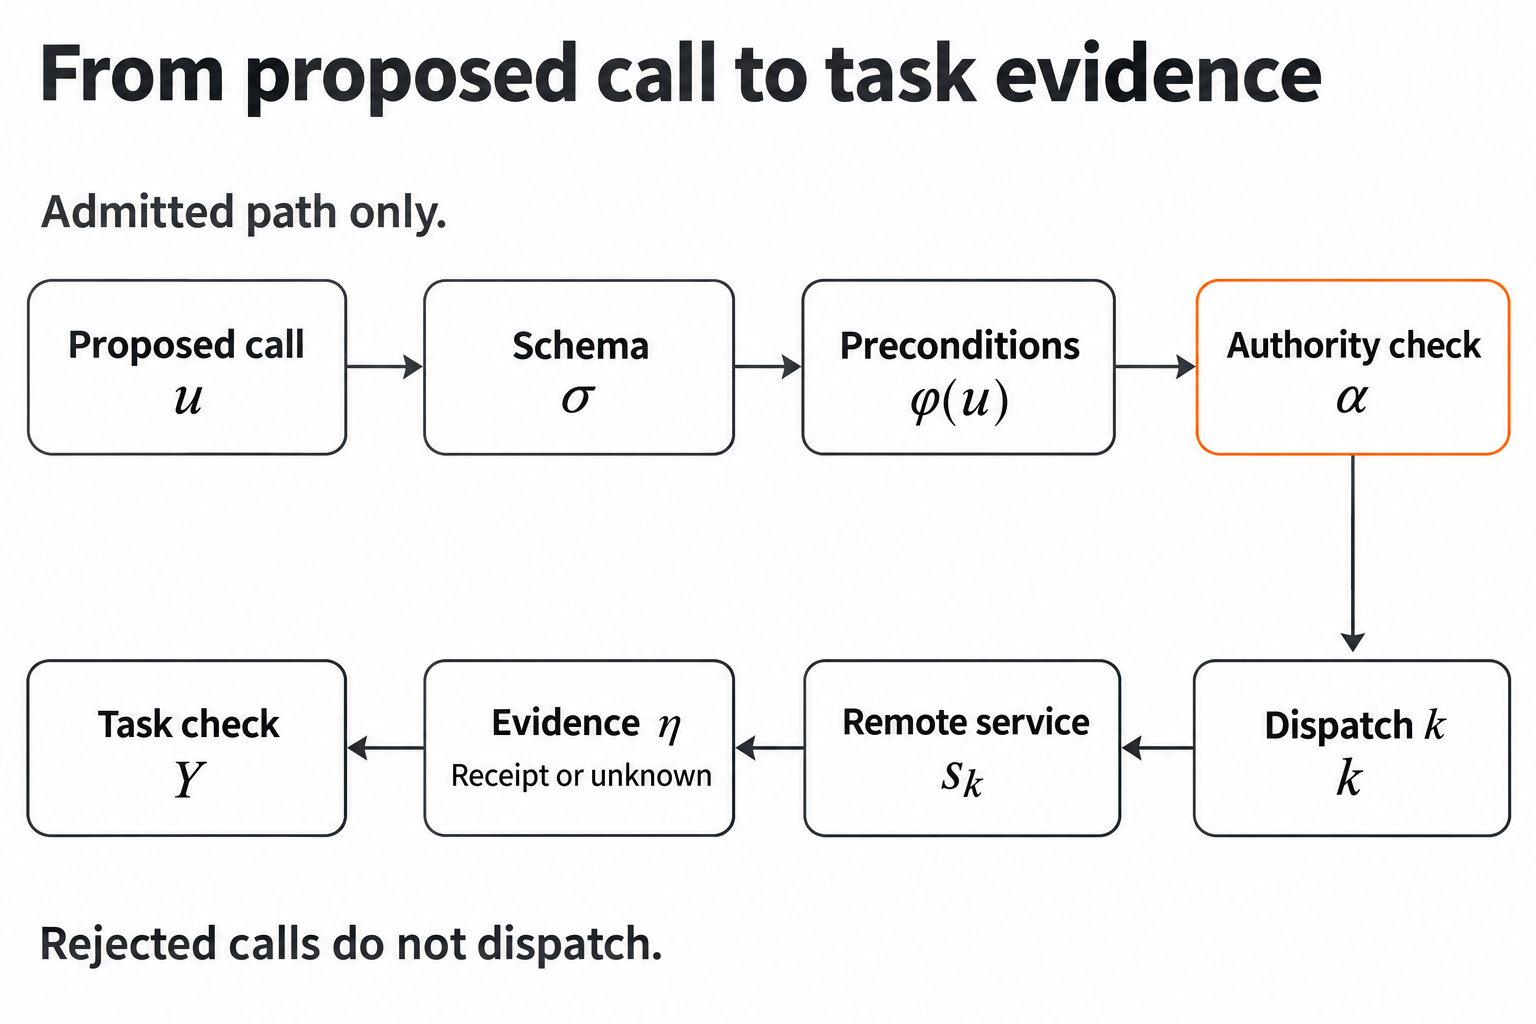
\includegraphics[width=\linewidth]{book/figures/assets/F18review.png}
\caption{A normative admitted tool path: schema, domain and current-authority checks precede dispatch. Here $\alpha$ denotes the authority epoch. Actual service evidence $\eta$, including unresolved outcomes, is recorded separately from a task check $Y$. This schematic does not claim that framework defaults enforce every boundary, that admission and remote commit are atomic, or that a receipt proves task correctness. Figure-local $\sigma$ names the schema, $\varphi(u)$ a domain predicate, $k$ the logical operation identifier, and $s_k$ its servicing endpoint.}
\label{fig:C18:overview}
\end{figure}
